\newif\ifen
\newif\ifes
\newcommand{\en}[1]{\ifen#1\fi}
\newcommand{\es}[1]{\ifes#1\fi}
\entrue
\usepackage[utf8]{inputenc}
\documentclass[a0,portrait]{a0poster} %A0 841mm x 1189mm
\usepackage{multicol} % This is so we can have multiple columns 
\columnsep=80pt % This is the amount of white space between the columns in the poster
\columnseprule=3pt % This is the thickness of the black line between the columns in the poster

\usepackage[svgnames]{xcolor} % Specify colors by their 'svgnames', for a full list of all colors available see here: http://www.latextemplates.com/svgnames-colors

%\usepackage{times} % Use the times font
%\usepackage{palatino} % Uncomment to use the Palatino font
%\usepackage[sfdefault]{AlegreyaSans}
\usepackage[sfdefault]{AlegreyaSans}

\usepackage{graphicx} % Required for including images
\graphicspath{{figures/}} % Location of the graphics files
\usepackage{booktabs} % Top and bottom rules for table
\usepackage[labelfont=bf]{caption} % Required for specifying captions to tables and figures
\usepackage{amsfonts, amsmath, amsthm, amssymb} % For math fonts, symbols and environments
\usepackage{wrapfig} % Allows wrapping text around tables and figures
\usepackage{bm}
\usepackage{ragged2e}
\usepackage{float} % para que los gr\'aficos se queden en su lugar con [H]
\usepackage[subrefformat=parens]{subcaption} % para \begin{subfigure}
\usepackage{tikz} % Para graficar, por ejemplo bayes networks
\usepackage{framed}
\usepackage{mdframed}
  
\usepackage[absolute,overlay]{textpos} 
\setlength{\TPHorizModule}{1cm} %
\setlength{\TPVertModule}{1cm}	%

\newcommand{\E}{\en{S}\es{E}}
\newcommand{\A}{\en{E}\es{A}}
\newcommand{\Ee}{\en{s}\es{e}}
\newcommand{\Aa}{\en{e}\es{a}}


\usetikzlibrary{bayesnet} % Para que ande se necesita copiar el archivo  tikzlibrarybayesnet.code.tex en la misma carpeta


\newcommand{\vm}[1]{\mathbf{#1}}
\newcommand{\N}{\mathcal{N}}
\newcommand\hfrac[2]{\genfrac{}{}{0pt}{}{#1}{#2}} %\frac{}{} sin la linea del medio

% \usepackage{xr}
% \externaldocument{supplementary}
\setlength{\columnseprule}{0pt}


\addtolength{\textwidth}{40pt}
\addtolength{\oddsidemargin}{-40pt}
 
\begin{document}
% 
% \begin{textblock}{100}(18,23.25)
%  \includegraphics[width=0.1\textwidth]{auxliar/images/dc_color.pdf} 
%  \end{textblock}
% \begin{textblock}{100}(30,24)
%  \includegraphics[width=0.1\textwidth]{auxliar/images/icc-logo.jpg} 
%  \end{textblock}
%  \begin{textblock}{100}(49,24)
%  \includegraphics[width=0.1\textwidth]{auxliar/images/logo_licar.pdf} 
%  \end{textblock}
%   \begin{textblock}{100}(61,24)
%  \includegraphics[width=0.1\textwidth]{auxliar/images/logo_version_02.pdf} 
%  \end{textblock}
%  
%----------------------------------------------------------------------------------------
%	POSTER HEADER 
%----------------------------------------------------------------------------------------

% The header is divided into two boxes:
% The first is 75% wide and houses the title, subtitle, names, university/organization and contact information
% The second is 25% wide and houses a logo for your university/organization or a photo of you
% The widths of these boxes can be easily edited to accommodate your content as you see fit
\centering \fontsize{90}{90} \textbf{Adaptative beliefs} \\[0.4cm]  % Title
\fontsize{70}{85}\textbf{Bayesian inference, evolution, and learning}\\[1cm] % Subtitle
\LARGE \textbf{Gustavo Landfried}  \ \ \  \texttt{glandfried@dc.uba.ar} \\
\large 1. Universidad de Buenos Aires. Facultad de Ciencias Exactas y Naturales. Departamento de Computaci\'on. Buenos Aires, Argentina \\ 
\large 2. CONICET-Universidad de Buenos Aires. Instituto de Investigaci\'on en Ciencias de la Computaci\'on (ICC). Buenos Aires, Argentina \\


 % A bit of extra whitespace between the header and poster content
\vspace{1cm}
%----------------------------------------------------------------------------------------


%\begin{paracol}{2}
\begin{multicols}{2}
% This is how many columns your poster will be broken into, a portrait poster is generally split into 2 columns













\fontsize{40}{50}\selectfont

\centrering

{\fontsize{60}{72}\selectfont \textbf{TrueSkill Through Time (TTT)} \\[0.2cm]
\LARGE \textbf{Reliable initial skill estimates and historical comparability} }

\justify 

\vspace{0.8cm}

\en{Unlike the most commonly used skill estimators in the video game industry (Elo, TrueSkill, Glicko), the TTT model obtains reliable initial skill estimates and guarantees historical comparability by propagating all historical information in a single Bayesian network. }%
\es{A diferencia de los estimadores de habilidad más utilizados en la industria del video juego (e.g Elo, TrueSkill, Glicko), el modelo TTT obtiene estimaciones fiables de la habilidad inicial y garantiza la comparabilidad histórica gracias a que propaga toda la información histórica en una única red bayesiana. }%
%
\en{In this paper we offer the first package for \texttt{Julia}, \texttt{Python} and \texttt{R}. }%
\es{En este artículo ofrecemos el primer paquete para \texttt{Julia}, \texttt{Python} y \texttt{R}. }%
%
\en{This algorithm requires few iterations to converge, allowing millions of observations to be analyzed using any low-end computer. }%
\es{Este algoritmo requiere pocas iteraciones para converger, permitiendo analizar millones de observaciones usando cualquier ordenador de gama baja. }

\section*{Introduction}
\begin{figure}[H]
  \centering
  \scalebox{1.66}{
      \tikz{         
    \node[det, fill=black!10] (r) {$r$} ; 
    \node[const, left=of r, xshift=-1.35cm] (r_name) {\small \en{Result}\es{Resultado}:}; 
    \node[const, right=of r] (dr) {$ r = (d > 0)$}; 

    \node[latent, above=of r, yshift=-1cm] (d) {$d$} ; %
    \node[const, right=of d] (dd) {$ d = p_i-p_j$}; 
    \node[const, left=of d, xshift=-1.35cm] (d_name) {\small \en{Difference}\es{Diferencia}:};
    
    \node[latent, above=of d, xshift=-1.5cm, yshift=-1cm] (p1) {$p_i$} ; %
    \node[latent, above=of d, xshift=1.5cm, yshift=-1cm] (p2) {$p_j$} ; %
    \node[const, left=of p1, xshift=-0.55cm] (p_name) {\small \en{Performance}\es{Desempeño}:}; 

    \node[accion, above=of p1,yshift=0.3cm] (s1) {} ; %
    \node[const, right=of s1] (ds1) {$s_i$};
    \node[accion, above=of p2,yshift=0.3cm] (s2) {} ; %
    \node[const, right=of s2] (ds2) {$s_j$};
    
    \node[const, right=of p2] (dp2) { $p \sim \N(s,\beta^2)$};

    \node[const, left=of s1, xshift=-.85cm] (s_name) {\small \en{Skill}\es{Habilidad}:}; 
    
    \edge {d} {r};
    \edge {p1,p2} {d};
    \edge {s1} {p1};
    \edge {s2} {p2};
    
 }
  }
  \caption{\small \emph{TrueSkill} acyclic Bayesian network model}
  \label{modelo_trueskill}
\end{figure}

\vspace{0.5cm}

\begin{figure}[H]
\centering
\scalebox{1.33}{
\tikz{
    \node[const] (a1) {\includegraphics[page=1,width=0.2\linewidth]{figures/trueskillthroughtime}};
    \node[const, left=of a1] (na) {\en{Player}\es{Jugador} A:};
    \node[const,right=of a1] (a2) {\includegraphics[page=2,width=0.2\linewidth]{figures/trueskillthroughtime}}; 
    \node[const,below=of a1] (b1) {\includegraphics[page=3,width=0.2\linewidth]{figures/trueskillthroughtime}}; 
    \node[const, left=of b1] (nb) {\en{Player}\es{Jugador} B:};
    \node[const,below=of a2] (b2) {\includegraphics[page=4,width=0.2\linewidth]{figures/trueskillthroughtime}}; 
    \node[const, above=of a1] (g1) {Game 1 ($p_A > p_B$)};
    \node[const, above=of a2] (g2) {Game 2 ($p_A < p_B$)};
    
}
}
\caption{
 \en{Estimates obtained with TrueSkill (red) and with TrueSkill Through Time (green) after having seen two players compete twice: the first time player A wins and the second time player B wins. }%
 \es{Estimaciones obtenidos con TrueSkill (rojo) y con TrueSkill Through Time (verde) luego de haber visto a dos jugadores competir dos veces: la primera gana el jugador A y en la segunda el jugador B. }%
}
\label{fig:trueskillthroughtime}
\end{figure}


\begin{figure}[H]
% \centering
\begin{subfigure}[b]{1\linewidth}
    \centering
    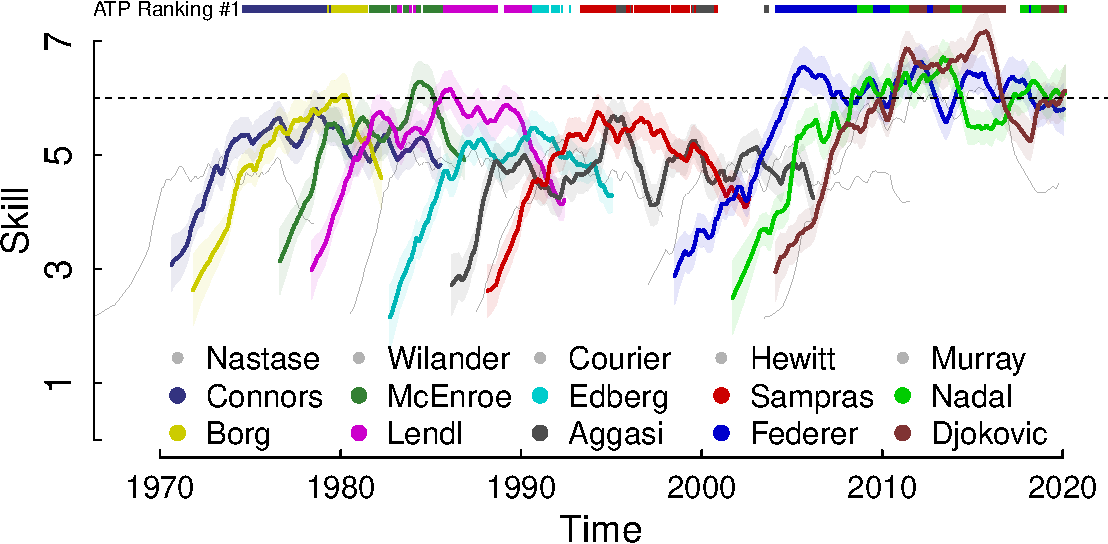
\includegraphics[width=.99\linewidth]{static/atp}
    \caption{
    \en{Estimated learning curves for some famous male players. }%
    \es{Curvas de aprendizaje estimadas de algunos jugadores masculinos. }%
    }
    \label{fig:atp}
\end{subfigure}
\end{figure}


\columnbreak



\centering

{\fontsize{60}{72}\selectfont \textbf{Evolutionary - Probabilistic isomorphism} \\[0.2cm]
\LARGE \textbf{The irreversible emergence of cooperation and specialization} }

\justify

\en{The reason why an advantage in favor of cooperation and specialization arises in our simple causal model is due to the multiplicative (non-ergodic) nature of probability theory and its isomorphism with evolutionary theory. }%
\es{El motivo por el cual surge una ventaja a favor de la cooperación y la especialización en este simple modelo causal se debe a la naturaleza multiplicativa (no-ergódica) de la teoría de la probabililidad y a su isomorfismo con la teoría de la evolución. }%



\begin{figure}[H]
    \centering
    \begin{subfigure}[b]{0.95\linewidth}
    \includegraphics[width=\linewidth]{auxiliar/images/biomass.jpg}
    \end{subfigure}
    \caption{
    \en{Distribution of biomass on Earth estimated by Bar-On et al.~\cite{barOn2018-biomass}. }
	\es{Distribución de la biomasa en la Tierra estimada por Bar-On et al.~\cite{barOn2018-biomass}. }%
    }
    \label{fig:biomass}
\end{figure}

\begin{equation} \label{eq:estrategia_base}
f(\Aa) =
\begin{cases}
 1.5 & \Aa = \text{ \en{Head}\es{Cara} } \\
 0.6 & \Aa = \text{ \en{Tail}\es{Sello} }
\end{cases}
\end{equation}


\begin{equation}
\begin{split}
\langle \omega_e \rangle_1 & = 1.5 \cdot \frac{1}{2} + 0.6 \cdot  \frac{1}{2} = 1.05
\end{split}
\end{equation}

\begin{figure}[H]
    \centering
    \begin{subfigure}[b]{0.49\linewidth}
    \includegraphics[width=\linewidth]{figures/pdf/ergodicity_expectedValue.pdf}
    \end{subfigure}
    \begin{subfigure}[b]{0.49\linewidth}
    \includegraphics[width=\linewidth]{figures/pdf/ergodicity_individual_trayectories.pdf}
    \end{subfigure}
\end{figure}

%
\begin{equation} \label{eq:geometric_mean}
\begin{split}
\lim_{T \rightarrow \infty} \omega_e(T) & = {g}^T \\
\left( \lim_{T \rightarrow \infty} \omega_e(T) \right)^{1/T} & =  {g} \\
\lim_{T \rightarrow \infty} f(\text{\en{head}\es{cara}})^{n_1/T} f(\text{\en{tail}\es{seca}})^{n_2/T} & 
 \end{split}
\end{equation}
%

% \begin{align*}
% \centering
%  \begin{tabular}{l|l}
%   \en{Bayes theorem}\es{Teorema de Bayes} & Replicator dynamic  \\ \hline
%   Prior $P(H)$ & \en{Old distribution of strategies}\es{Distribución de estrategias} $x_\Ee$ \\ \hline
%   \en{Likelihood}\es{Verosimilitud} $P(D|H)$ & \en{Fitness}\es{Aptitud} $f_\Ee(\Aa)$ \\ \hline
%   Posterior $P(H|D)$ & \en{New distribution of strategies}\es{Nueva distribución de estrategias} $x_\Ee^\prime$ \\ \hline
%   Evidenc\en{e}\es{ia} $P(D)$ & \en{Population mean fitness}\es{Aptitud media de la población} $\sum_\Ee x_\Ee f_\Ee(\Aa) $ \\ \hline
%  \end{tabular}
% \end{align*}

\begin{figure}[H]
    \centering
    \begin{subfigure}[b]{0.49\linewidth}
    \includegraphics[width=\linewidth]{figures/pdf/tasa-temporal-0.pdf}
    \end{subfigure}
    \begin{subfigure}[b]{0.49\linewidth}
    \includegraphics[width=\linewidth]{figures/pdf/tasa-temporal-2.pdf}
    \end{subfigure}
    \label{fig:tasa-temporal-2}
\end{figure}









\end{multicols}
{ \footnotesize
%\nocite{*} % Print all references regardless of whether they were cited in the poster or not
\bibliographystyle{./biblio/plos2015} % Plain referencing style
\bibliography{./biblio/biblio.bib} % Use the example bibliography file sample.bib
}
\end{document}
